\documentclass[a4paper,12pt]{article}
\usepackage[margin=1in]{geometry}
\usepackage{tikz}
\usetikzlibrary{shapes,arrows}

\title{Regression Interpretation Activity}
\author{}
\date{}

\begin{document}
	
\maketitle

\vspace{-2em}
	
\section*{Purpose}

This activity is intended to improve your ability to interpret regression estimates, fitted values, and the marginal effect of variables included in complex regression models. For each of the following regression equations, please draw (by hand) the fitted regression surface according to the equation and instructions provided.

\section{Ordinary Least Squares}

In this equation, we are predicting life satisfaction as a function of years of education and gender. The estimated model is as follows:

\begin{equation}
\hat{y} = 2 + 0.2 x + (-1.5 z)
\end{equation}

\noindent where $x$ is years of post-secondary education (from 0 to 8), and $z$ is an indicator for being female. Please draw this fitted regression surface in the space provided below. 

\begin{center}
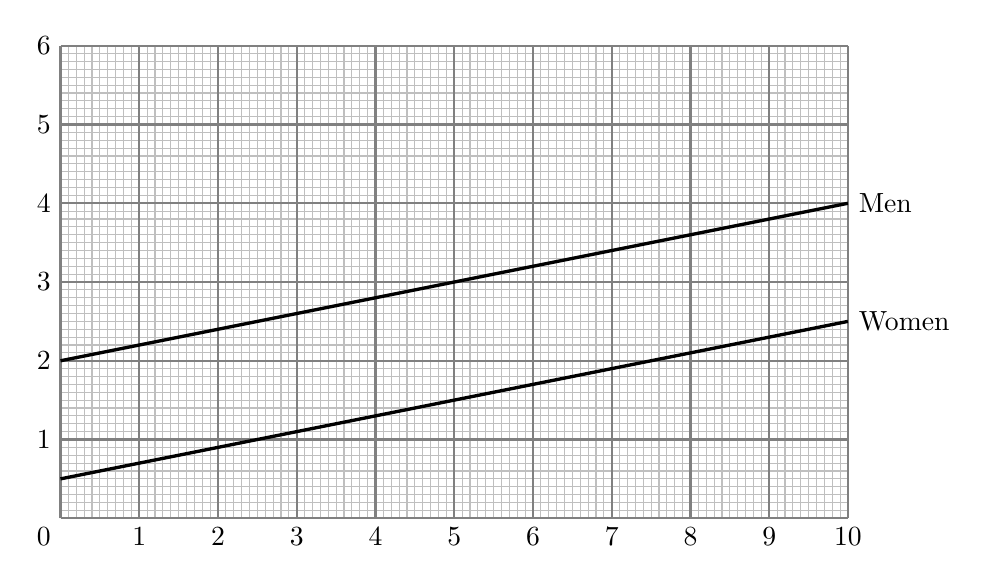
\begin{tikzpicture}
\draw [thin, step=0.1, lightgray] (0,0) grid (10,6);
\draw [thick, gray] (0,0) grid (10,6);
\node[below left] () at (0,0) {0};
\foreach \x in {1,...,10} {
    \node[below] () at (\x,0) {\x};
}
\foreach \y in {1,...,6} {
    \node[left] () at (0,\y) {\y};
}
% answer for men
\draw [very thick, black] (0,2) -- (10,4) node[right] {Men};
% answer for women
\draw [very thick, black] (0,0.5) -- (10,2.5) node[right] {Women};
\end{tikzpicture}
\end{center}

\noindent Then, for the values $x \in \{0,4,8\}$, calculate the \textbf{marginal effect} of $x$ (education) on $y$ and the \textbf{marginal effect} of $z$ (being female) on $y$.


\clearpage

\section{Ordinary Least Squares (with Interaction)}

In this equation, we are predicting life satisfaction as a function of years of education, separately for men and women. The estimated model is as follows:

\begin{equation}
\hat{y} = 2 + 0.2 x + (-1.5 z) + 0.25 x*z
\end{equation}

\noindent where $x$ is years of post-secondary education (from 0 to 8) and $z$ is an indicator for being female. Please draw this fitted regression surface in the space provided below. 

\begin{center}
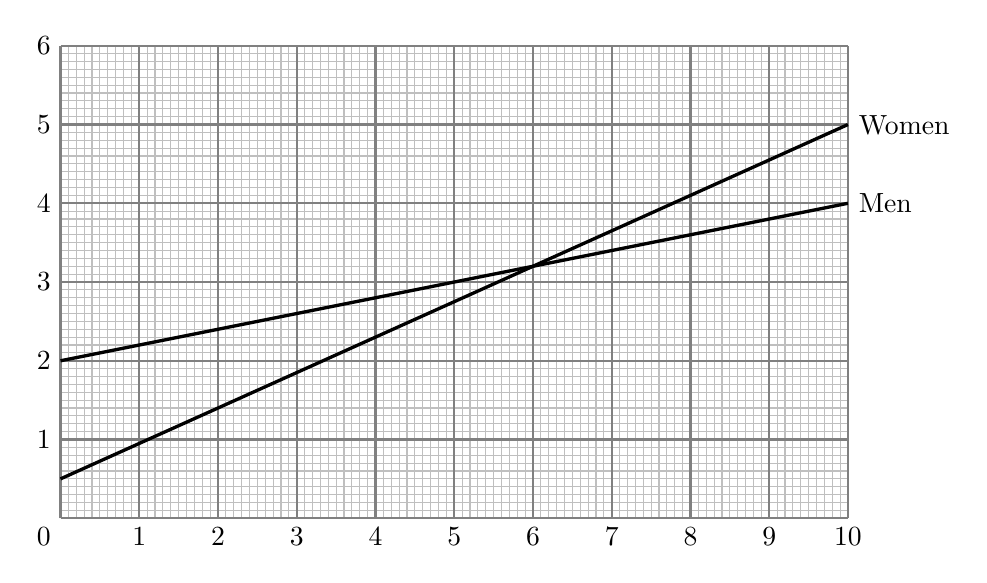
\begin{tikzpicture}
\draw [thin, step=0.1, lightgray] (0,0) grid (10,6);
\draw [thick, gray] (0,0) grid (10,6);
\node[below left] () at (0,0) {0};
\foreach \x in {1,...,10} {
    \node[below] () at (\x,0) {\x};
}
\foreach \y in {1,...,6} {
    \node[left] () at (0,\y) {\y};
}
% answer for men
\draw [very thick, black] (0,2) -- (10,4) node[right] {Men};
% answer for women
\draw [very thick, black] (0,0.5) -- (10,5) node[right] {Women};
\end{tikzpicture}
\end{center}

\noindent Then, for the values $x \in \{0,2,4,6,8\}$ and $z \in \{0,1\}$, calculate the \textbf{marginal effects} of both $x$ and $z$ on $y$. Draw both marginal effect in the space below.

\begin{center}
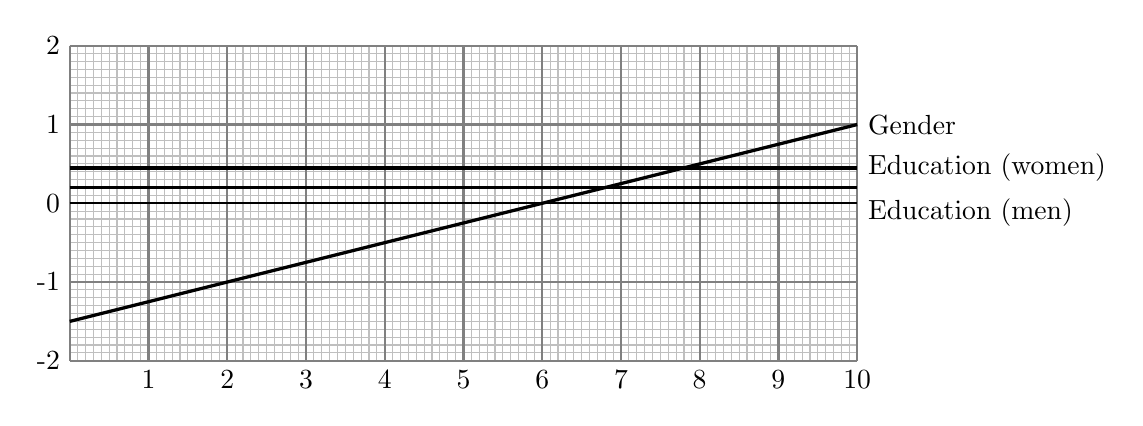
\begin{tikzpicture}
\draw [thin, step=0.1, lightgray] (0,-2) grid (10,2);
\draw [thick, gray] (0,-2) grid (10,2);
\draw [thick, black] (0,0) grid (10,0);
\foreach \x in {1,...,10} {
    \node[below] () at (\x,-2) {\x};
}
\foreach \y in {-2,...,2} {
    \node[left] () at (0,\y) {\y};
}
% marginal effect of being female
\draw [very thick, black] (0,-1.5) -- (10,1) node[right] {Gender};
% marginal effects of education
\draw [very thick, black] (0,0.2) -- (10,0.2) node[below right] {Education (men)};
\draw [very thick, black] (0,0.45) -- (10,0.45) node[right] {Education (women)};
\end{tikzpicture}
\end{center}





\clearpage

\section{Ordinary Least Squares (with Non-Linear Term)}

In this equation, we are predicting life satisfaction as a function of years of education. The estimated model is as follows:

\begin{equation}
\hat{y} = 5 - x + 0.1 x^2
\end{equation}

\noindent where $x$ is years of post-secondary education (from 0 to 8). Please draw this fitted regression surface in the space provided below. 

\begin{center}
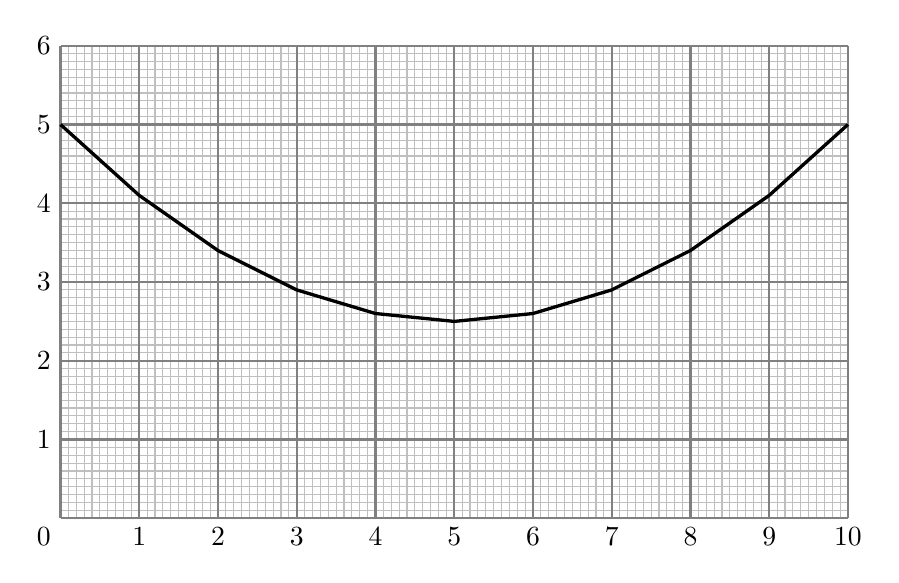
\begin{tikzpicture}
\draw [thin, step=0.1, lightgray] (0,0) grid (10,6);
\draw [thick, gray] (0,0) grid (10,6);
\node[below left] () at (0,0) {0};
\foreach \x in {1,...,10} {
    \node[below] () at (\x,0) {\x};
}
\foreach \y in {1,...,6} {
    \node[left] () at (0,\y) {\y};
}
% answer
\draw [very thick, black] (0,5) -- (1,4.1) -- (2,3.4) -- (3, 2.9) -- (4,2.6) -- (5,2.5) -- (6,2.6) -- (7,2.9) -- (8,3.4) -- (9,4.1) -- (10,5);
\end{tikzpicture}
\end{center}

\noindent Then, for the values $x \in \{0,1,...,10\}$, calculate the \textbf{marginal effect} of $x$ on $y$. Draw this marginal effect in the space below.

\begin{center}
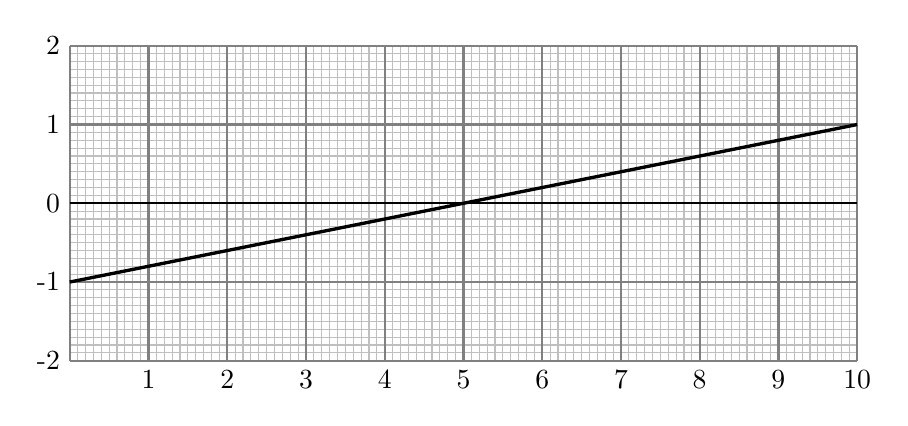
\begin{tikzpicture}
\draw [thin, step=0.1, lightgray] (0,-2) grid (10,2);
\draw [thick, gray] (0,-2) grid (10,2);
\draw [thick, black] (0,0) grid (10,0);
\foreach \x in {1,...,10} {
    \node[below] () at (\x,-2) {\x};
}
\foreach \y in {-2,...,2} {
    \node[left] () at (0,\y) {\y};
}
% marginal effect of x ($0.2 x - 1$)
\draw [very thick, black] (0,-1) -- (10,1);
\end{tikzpicture}
\end{center}



\clearpage

\section{Logistic Regression with One Variable}

In this equation, we are predicting the probability of expressing satisfaction with life (life satisfaction is 1 rather than 0) as a function of years of education. The estimated model is as follows:

\begin{equation}
Pr(y = 1) = f(\hat{y\ast}) = f(-5 + x)
\end{equation}

\noindent where $x$ is years of post-secondary education (from 0 to 8) and $f()$ is the logit function. This fitted regression surface is provided in the space below. 

\begin{center}
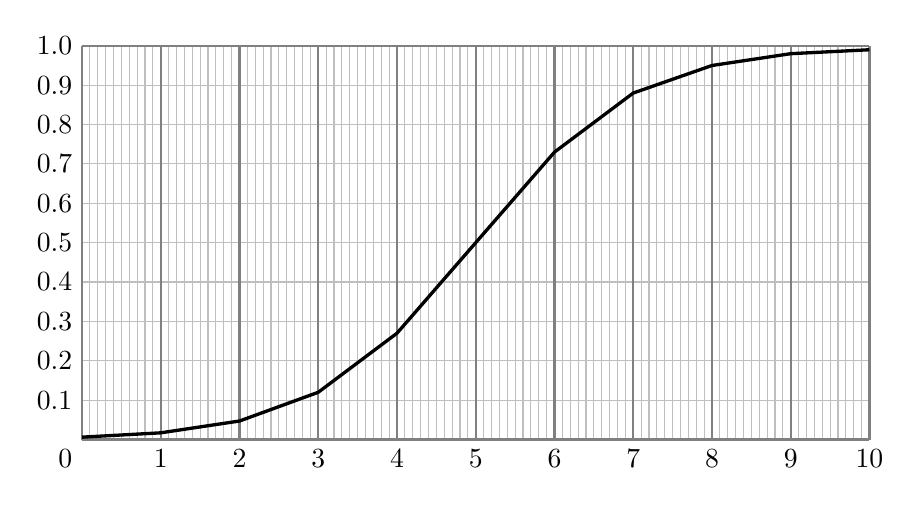
\begin{tikzpicture}[yscale=5]
\draw [thin, step=0.1, lightgray] (0,0) grid (10,1);
\draw [thick, gray] (0,0) grid (10,1);
\node[below left] () at (0,0) {0};
\foreach \x in {1,...,10} {
    \node[below] () at (\x,0) {\x};
}
\foreach \y in {0.1,0.2,0.3,0.4,0.5,0.6,0.7,0.8,0.9,1.0} {
\node[left] () at (0,\y) {\y};
}
\draw [very thick, black] (0,0.006) -- (1,0.017) -- (2,0.047) -- (3,0.12) -- (4,0.27) -- (5,0.5) -- (6,0.73) -- (7,0.88) -- (8,0.95) -- (9,0.98) -- (10,0.99);
\end{tikzpicture}
\end{center}

\noindent For the values $x \in \{0,1,...,10\}$, calculate the \textbf{marginal effect} of $x$ on $y$. Draw this marginal effect curve in the space below.

\begin{center}
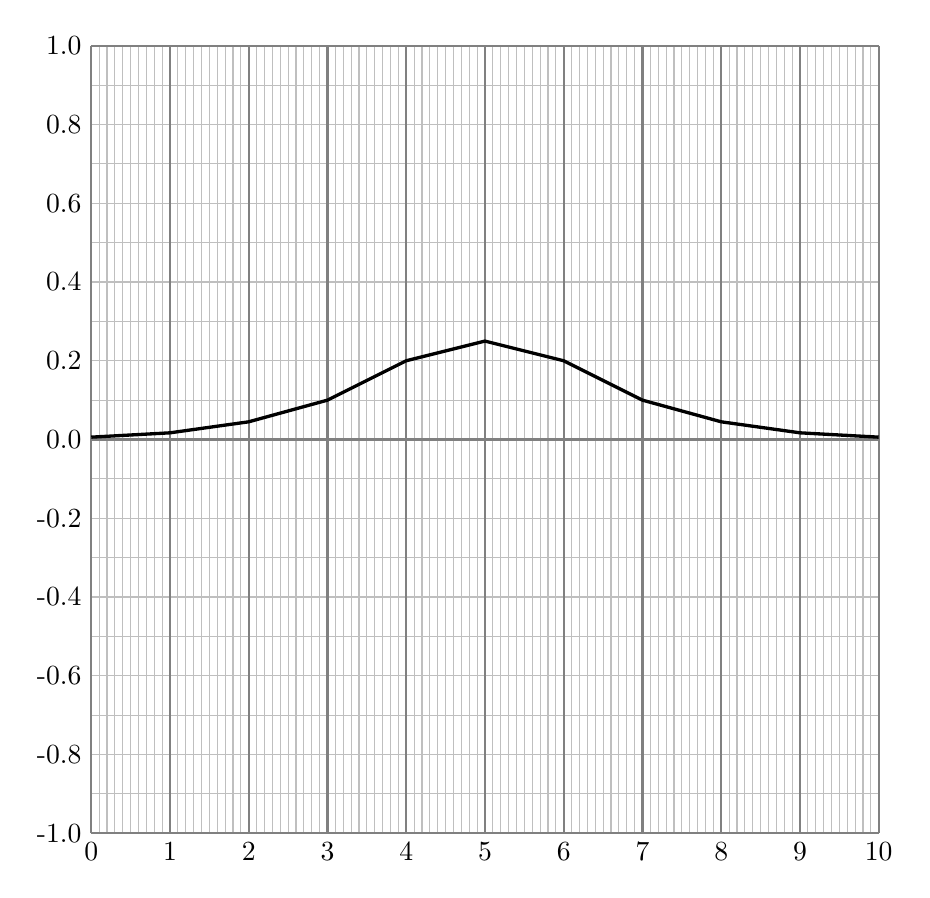
\begin{tikzpicture}[yscale=5]
\draw [thin, step=0.1, lightgray] (0,-1) grid (10,1);
\draw [thick, gray] (0,-1) grid (10,1);
\foreach \x in {0,...,10} {
    \node[below] () at (\x,-1) {\x};
}
\foreach \y in {-1.0,-0.8,-0.6,-0.4,-0.2,0.0,0.2,0.4,0.6,0.8,1.0} {
\node[left] () at (0,\y) {\y};
}
% marginal effect of x (dlogis)
\draw [very thick, black] (0,0.006) -- (1,0.017) -- (2,0.045) -- (3,0.10) -- (4,0.20) -- (5,0.25) -- (6,0.20) -- (7,0.10) -- (8,0.045) -- (9,0.017) -- (10,0.006);
\end{tikzpicture}
\end{center}


\section{Logistic Regression with Discrete Effect}

In this equation, we are predicting the probability of expressing satisfaction with life (life satisfaction is 1 rather than 0) as a function of years of education and gender. The estimated model is as follows:

\begin{equation}
Pr(y = 1) = f(\hat{y\ast}) = f(-5 + x + 2 z)
\end{equation}

\noindent where $x$ is years of post-secondary education (from 0 to 8), $z$ is an indicator for being female, and $f()$ is the logit function. This fitted regression surface is provided in the space below. Which line represents men and which line represents women?

\begin{center}
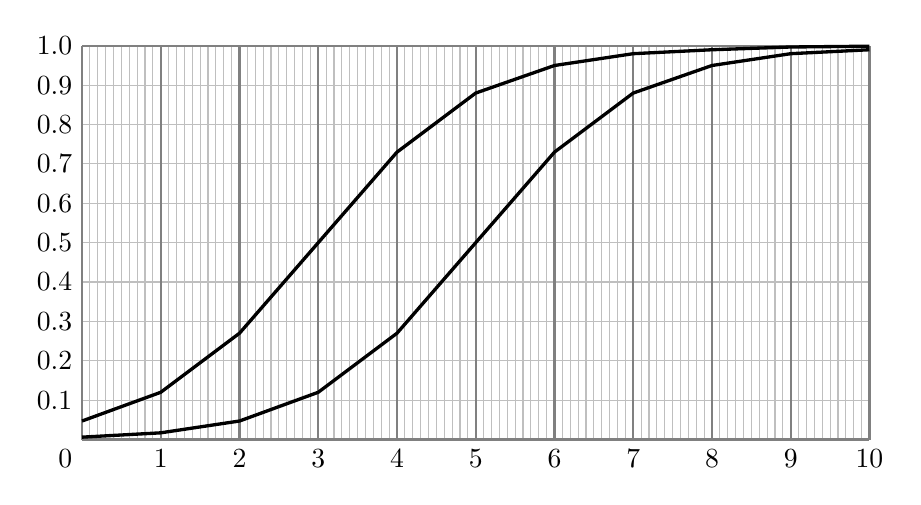
\begin{tikzpicture}[yscale=5]
\draw [thin, step=0.1, lightgray] (0,0) grid (10,1);
\draw [thick, gray] (0,0) grid (10,1);
\node[below left] () at (0,0) {0};
\foreach \x in {1,...,10} {
    \node[below] () at (\x,0) {\x};
}
\foreach \y in {0.1,0.2,0.3,0.4,0.5,0.6,0.7,0.8,0.9,1.0} {
\node[left] () at (0,\y) {\y};
}
\draw [very thick, black] (0,0.006) -- (1,0.017) -- (2,0.047) -- (3,0.12) -- (4,0.27) -- (5,0.5) -- (6,0.73) -- (7,0.88) -- (8,0.95) -- (9,0.98) -- (10,0.99);
\draw [very thick, black] (0,0.047) -- (1,0.12) -- (2,0.27) -- (3,0.5) -- (4,0.73) -- (5,0.88) -- (6,0.95) -- (7,0.98) -- (8,0.99) -- (9,0.997) -- (10,0.999);
\end{tikzpicture}
\end{center}

\noindent For the values $x \in \{0,1,...,10\}$, calculate the \textbf{marginal effect} of $z$ on $y$. Note that for a discrete variable, the we often calculate a \textit{discrete} change between categories rather than the instantaneous marginal effect. Draw this discrete effect curve in the space below.

\begin{center}
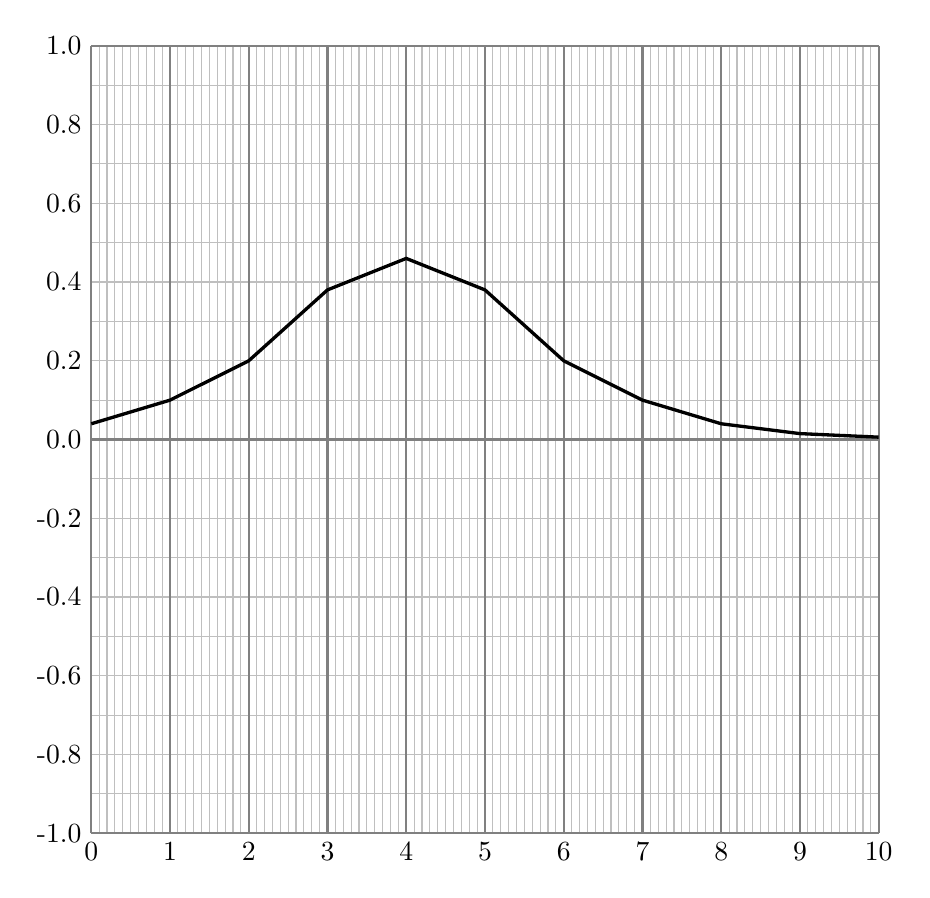
\begin{tikzpicture}[yscale=5]
\draw [thin, step=0.1, lightgray] (0,-1) grid (10,1);
\draw [thick, gray] (0,-1) grid (10,1);
\foreach \x in {0,...,10} {
    \node[below] () at (\x,-1) {\x};
}
\foreach \y in {-1.0,-0.8,-0.6,-0.4,-0.2,0.0,0.2,0.4,0.6,0.8,1.0} {
\node[left] () at (0,\y) {\y};
}
% marginal effect of x (dlogis)
\draw [very thick, black] (0,0.04) -- (1,0.10) -- (2,0.2) -- (3,0.38) -- (4,0.46) -- (5,0.38) -- (6,0.2) -- (7,0.10) -- (8,0.04) -- (9,0.015) -- (10,0.006);
\end{tikzpicture}
\end{center}

\section{Logistic Regression with Covariates}

\noindent An important difference between marginal effects in linear models (OLS) compared to generalized linear models relates to how covariates in the model affect the marginal effect estimate. In OLS, the marginal effect of $x$ does not depend on the values of $z$ unless there is an explicit interaction terms. In generalized linear models, this is not the case.\\

\noindent Using the same example regression equation as the previous example ($f(-5 + x + 2z)$), draw the marginal effects of $x$ when $z = 0$ and when $z = 1$. In the first space below, assume that $f()$ is the identity function:

\begin{center}
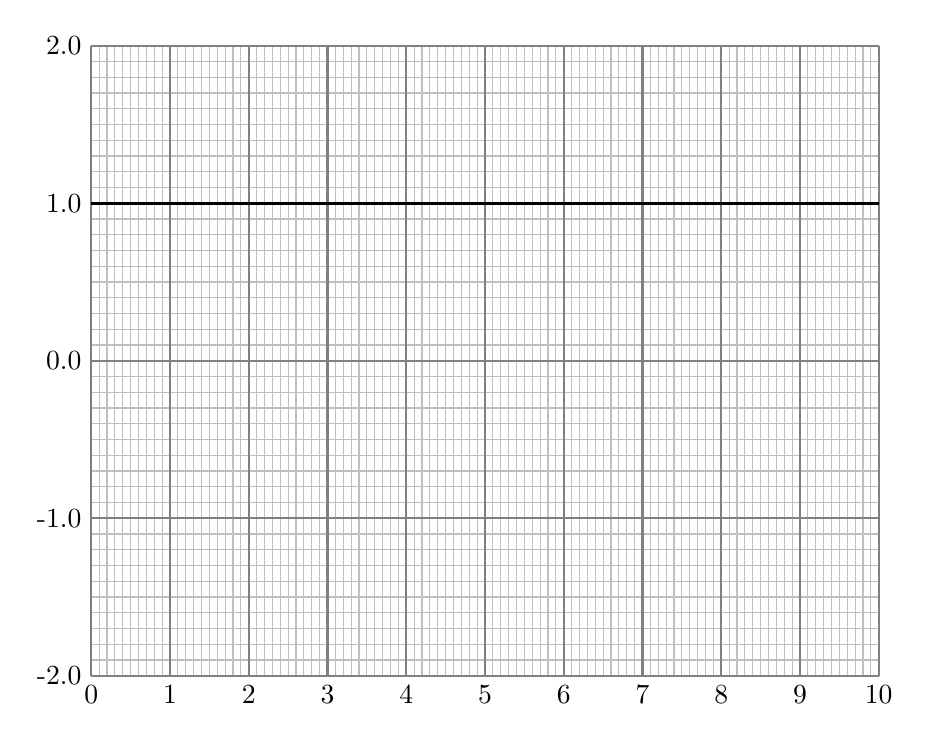
\begin{tikzpicture}[yscale=2]
\draw [thin, step=0.1, lightgray] (0,-2) grid (10,2);
\draw [thick, gray] (0,-2) grid (10,2);
\foreach \x in {0,...,10} {
    \node[below] () at (\x,-2) {\x};
}
\foreach \y in {-2.0, -1.0, 0.0, 1.0, 2.0} {
\node[left] () at (0,\y) {\y};
}
% marginal effect of x
\draw [very thick, black] (0,1) -- (10,1);
\end{tikzpicture}
\end{center}

 
\noindent Now assume that $f()$ is the logistic function (i.e., use the predicted probability plots on the previous page to estimate the marginal effects)
 
 
\begin{center}
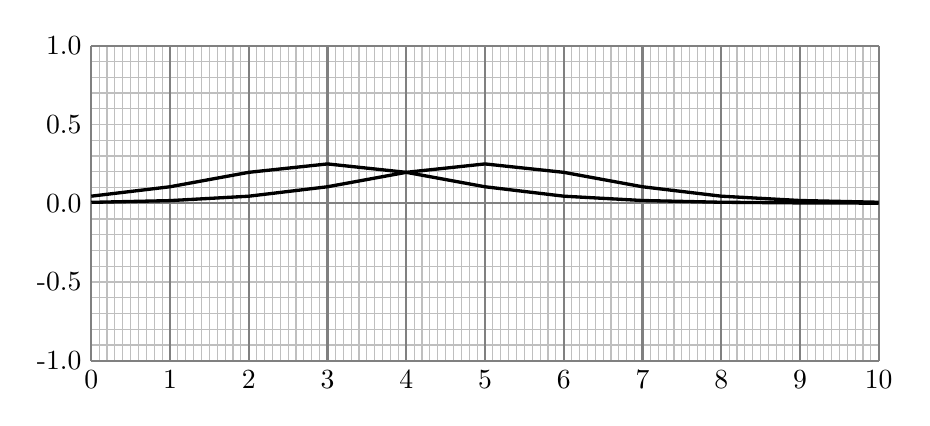
\begin{tikzpicture}[yscale=2]
\draw [thin, step=0.1, lightgray] (0,-1.0) grid (10,1);
\draw [thick, gray] (0,-1.0) grid (10,1);
\foreach \x in {0,...,10} {
    \node[below] () at (\x,-1.0) {\x};
}
\foreach \y in {-1.0, -0.5, 0.0, 0.5, 1.0} {
\node[left] () at (0,\y) {\y};
}
% marginal effect of x (dlogis) for men
\draw [very thick, black] (0,0.006) -- (1,0.017) -- (2,0.045) -- (3,0.105) -- (4,0.1966) -- (5,0.25) -- (6,0.1966) -- (7,0.10499) -- (8,0.04518) -- (9,0.01766) -- (10,0.0066);
% marginal effect of x (dlogis) for women
\draw [very thick, black] (0,0.0452) -- (1,0.105) -- (2,0.1966) -- (3,0.25) -- (4,0.1966) -- (5,0.10499) -- (6,0.04518) -- (7,0.01766) -- (8,0.0066) -- (9,0.0025) -- (10,0.0009);
\end{tikzpicture}
\end{center}



\clearpage
\section{Logistic Regression with Interaction}

In this equation, we are predicting the probability of expressing satisfaction with life (life satisfaction is 1 rather than 0) as a function of years of education and gender. The estimated model is as follows:

\begin{equation}
Pr(y = 1) = f(\hat{y\ast}) = f(-5 + x + 2 z - x*z)
\end{equation}

\noindent where $x$ is years of post-secondary education (from 0 to 8), $z$ is an indicator for being female, and $f()$ is the logit function. This fitted regression surface is provided in the space below. Which line represents men and which line represents women?

\begin{center}
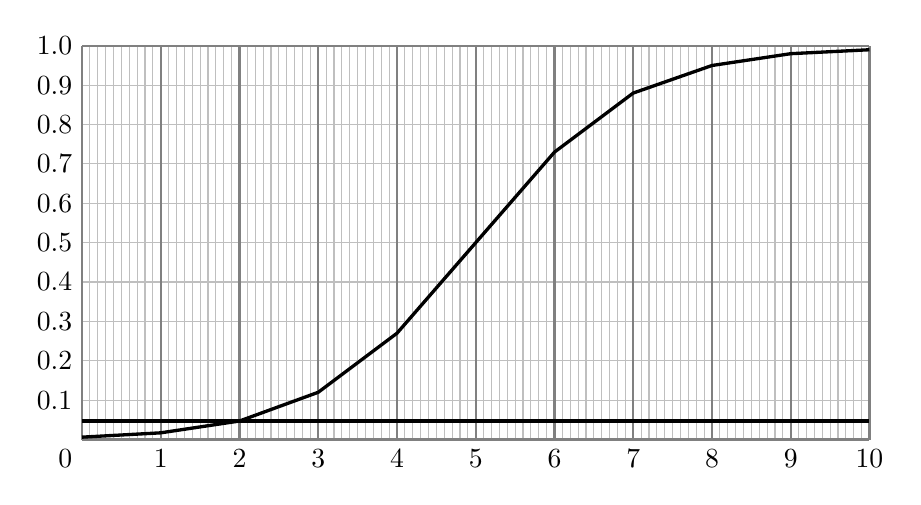
\begin{tikzpicture}[yscale=5]
\draw [thin, step=0.1, lightgray] (0,0) grid (10,1);
\draw [thick, gray] (0,0) grid (10,1);
\node[below left] () at (0,0) {0};
\foreach \x in {1,...,10} {
    \node[below] () at (\x,0) {\x};
}
\foreach \y in {0.1,0.2,0.3,0.4,0.5,0.6,0.7,0.8,0.9,1.0} {
\node[left] () at (0,\y) {\y};
}
\draw [very thick, black] (0,0.006) -- (1,0.017) -- (2,0.047) -- (3,0.12) -- (4,0.27) -- (5,0.5) -- (6,0.73) -- (7,0.88) -- (8,0.95) -- (9,0.98) -- (10,0.99);
\draw [very thick, black] (0,0.0474) -- (10,0.0474);
\end{tikzpicture}
\end{center}

\noindent For the values $x \in \{0,1,...,10\}$ and $z \in \{0,1\}$, calculate the \textbf{marginal effects} of $x$ and $z$ on $y$. Draw these curves below

\begin{center}
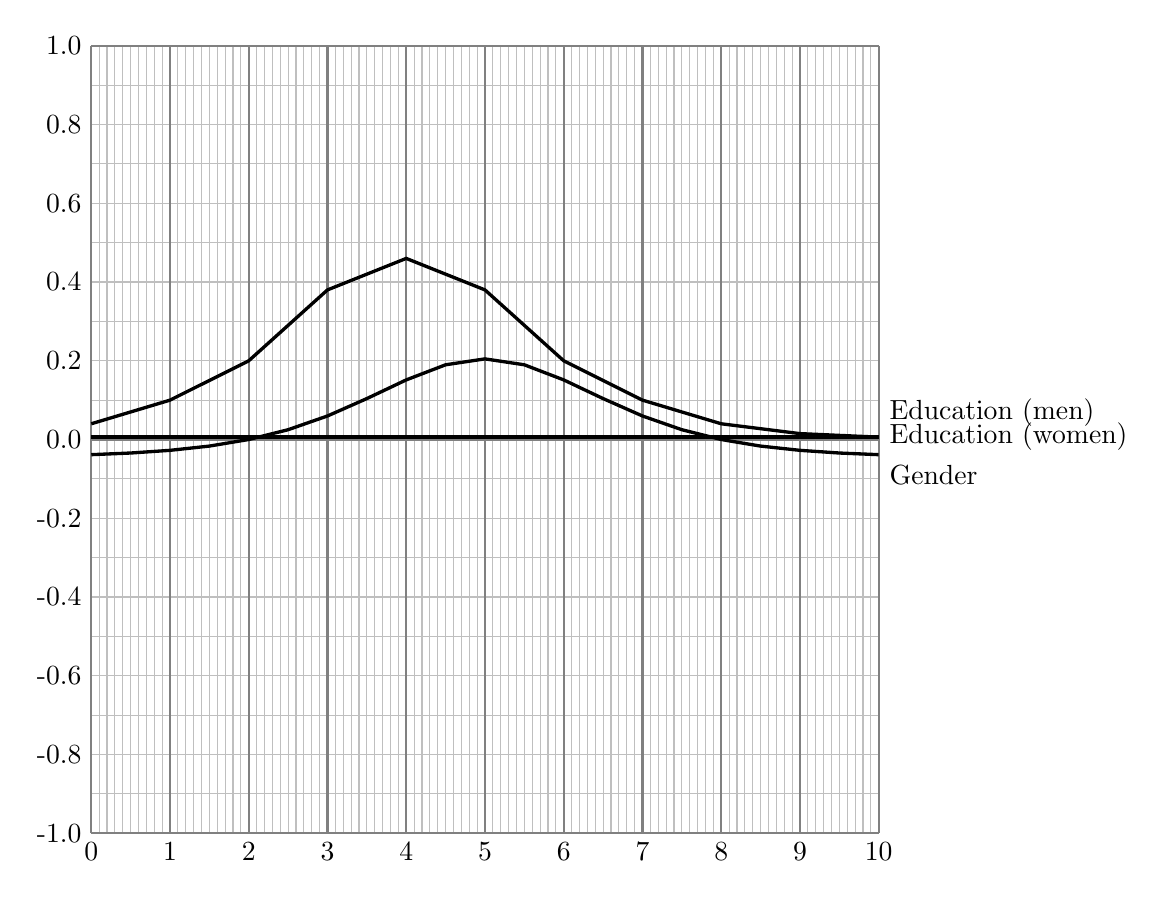
\begin{tikzpicture}[yscale=5]
\draw [thin, step=0.1, lightgray] (0,-1) grid (10,1);
\draw [thick, gray] (0,-1) grid (10,1);
\foreach \x in {0,...,10} {
    \node[below] () at (\x,-1) {\x};
}
\foreach \y in {-1.0,-0.8,-0.6,-0.4,-0.2,0.0,0.2,0.4,0.6,0.8,1.0} {
\node[left] () at (0,\y) {\y};
}
% marginal effect of z
% paste0("(", seq(0,10,by=0.5), ",", round(dlogis(-5 + (seq(0,10,by=0.5))) - dlogis(-3),4), ")", collapse = " -- ")
\draw [very thick, black] (0,-0.0385) -- (0.5,-0.0343) -- (1,-0.0275) -- (1.5,-0.0167) -- (2,0) -- (2.5,0.0249) -- (3,0.0598) -- (3.5,0.104) -- (4,0.1514) -- (4.5,0.1898) -- (5,0.2048) -- (5.5,0.1898) -- (6,0.1514) -- (6.5,0.104) -- (7,0.0598) -- (7.5,0.0249) -- (8,0) -- (8.5,-0.0167) -- (9,-0.0275) -- (9.5,-0.0343) -- (10,-0.0385) node[below right] {Gender};
% marginal effect of x for men
\draw [very thick, black] (0,0.04) -- (1,0.10) -- (2,0.2) -- (3,0.38) -- (4,0.46) -- (5,0.38) -- (6,0.2) -- (7,0.10) -- (8,0.04) -- (9,0.015) -- (10,0.006) node[above right] {Education (men)};
% marginal effect of x for women
\draw [very thick, black] (0,0.0066) -- (10,0.0066) node[right] {Education (women)};
\end{tikzpicture}
\end{center}


\section{Logit versus Probit}

The numeric values of coefficients in the logit and probit models differ from one another considerably, but tend to produce very similar inferences. Consider, again, the one-variable regression from above:

\begin{equation}
Pr(y = 1) = f(\hat{y\ast}) = f(-5 + x)
\end{equation}

\noindent where $x$ is years of post-secondary education (from 0 to 8) and $f()$ is the logit function. This fitted regression surface is provided in the space below:

\begin{center}
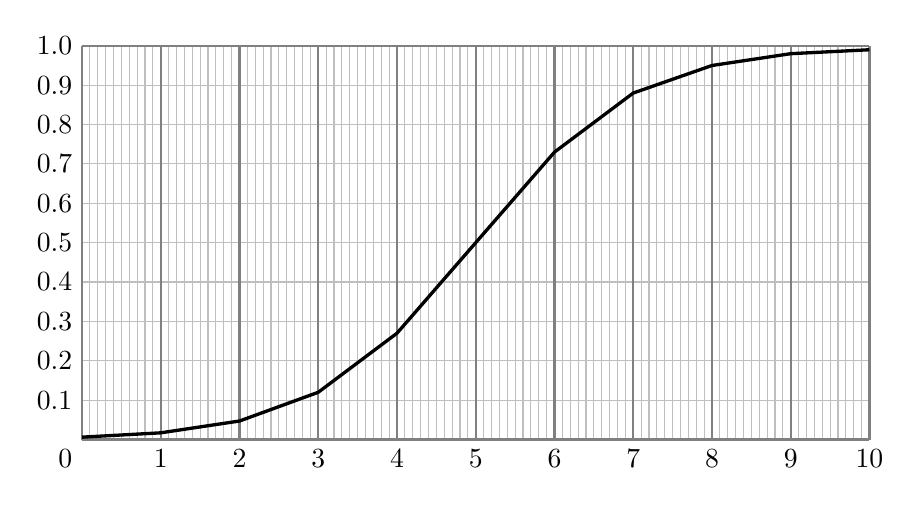
\begin{tikzpicture}[yscale=5]
\draw [thin, step=0.1, lightgray] (0,0) grid (10,1);
\draw [thick, gray] (0,0) grid (10,1);
\node[below left] () at (0,0) {0};
\foreach \x in {1,...,10} {
    \node[below] () at (\x,0) {\x};
}
\foreach \y in {0.1,0.2,0.3,0.4,0.5,0.6,0.7,0.8,0.9,1.0} {
\node[left] () at (0,\y) {\y};
}
\draw [very thick, black] (0,0.006) -- (1,0.017) -- (2,0.047) -- (3,0.12) -- (4,0.27) -- (5,0.5) -- (6,0.73) -- (7,0.88) -- (8,0.95) -- (9,0.98) -- (10,0.99);
\end{tikzpicture}
\end{center}

\noindent Here is another version of the same model, where $g()$ is the cumulative normal distribution function:

\begin{equation}
Pr(y = 1) = g(\hat{y\ast}) = g(-3.125 + 0.625 x)
\end{equation}

\noindent This regression surface is provided below:

\begin{center}
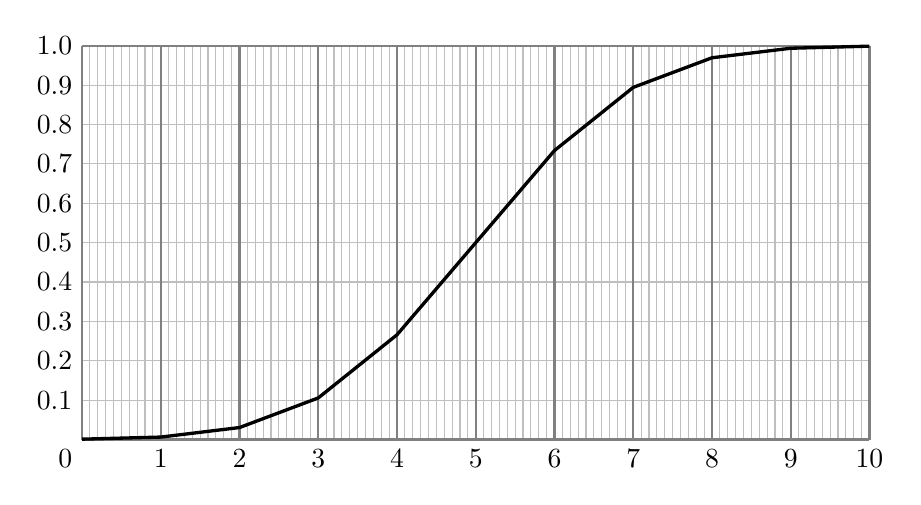
\begin{tikzpicture}[yscale=5]
\draw [thin, step=0.1, lightgray] (0,0) grid (10,1);
\draw [thick, gray] (0,0) grid (10,1);
\node[below left] () at (0,0) {0};
\foreach \x in {1,...,10} {
    \node[below] () at (\x,0) {\x};
}
\foreach \y in {0.1,0.2,0.3,0.4,0.5,0.6,0.7,0.8,0.9,1.0} {
\node[left] () at (0,\y) {\y};
}
\draw [very thick, black] (0,0.0009) -- (1,0.0062) -- (2,0.0304) -- (3,0.1056) -- (4,0.2660) -- (5,0.5) -- (6,0.7340) -- (7,0.8944) -- (8,0.9696) -- (9,0.9938) -- (10,0.9991);
\end{tikzpicture}
\end{center}

\noindent How do the marginal effects of $x$ in the logit and probit specifications compare?





\end{document}